
	
	
	\begin{document}
		
		
		
	This section details the experimental implementation of an actively loaded differential amplifier with a common source output, cascoded current mirror and a class B amplifier stage at the output. These also include components for frequency compensation and a load.The power supplies and analysis were implemented using the Digilent Analog Discovery kit. The experimental circuit can be seen Figure \ref{fig:expercircuit}.
		
		
				
		\begin{figure}[H]
			\begin{center}
				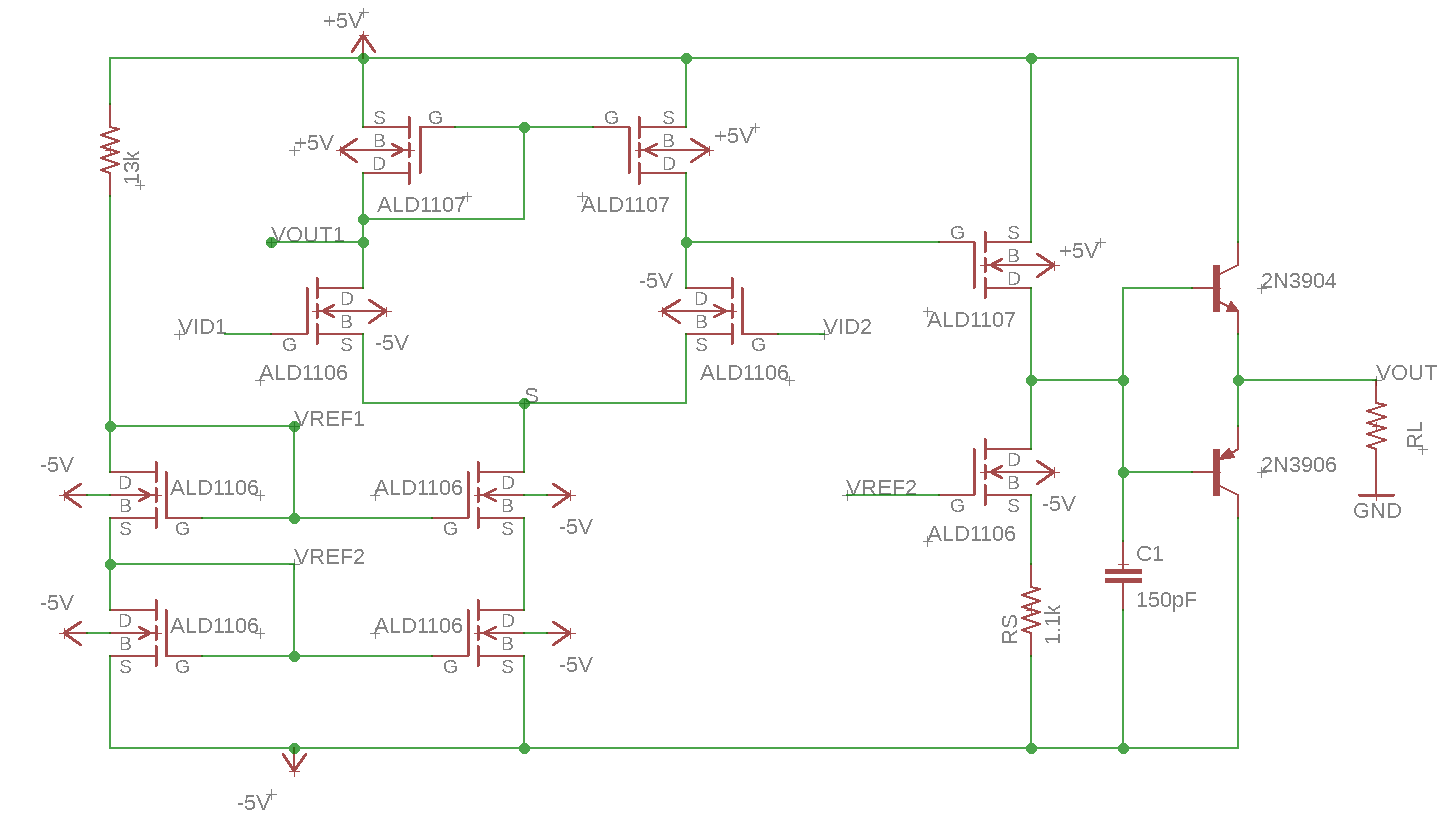
\includegraphics[scale=.40]{ExperimentalImplementation/expschem.png}
				\caption{Experimental range of operation}
				\label{fig:expercircuit}
			\end{center}
		\end{figure}

	
	The DC bias conditions were measured using a DT830B DVM. Nodal voltages were measured in reference to ground and current was measured by wiring the DVM in series while in ammeter mode. The bias conditions were measured while both input nodes to the circuit were grounded. The final measured values can be seen in Table \ref{tab:expdc}.
		
		
		\begin{table}[H]
			\centering
			\caption{Experimental DC values}
			\label{tab:expdc}
			\begin{tabular}{|l|l|}
				\hline
				\textbf{DC Bias Conditions} &           \\ \hline
				V$_{Ref_1}$                        & -3.01 V   \\ \hline
				V$_{Ref_2}$                        & -403 mV \\ \hline
				D1                          & 2.82 V     \\ \hline
				D2                          & 2.84 V     \\ \hline
				S                           & 2 V    \\ \hline
				OutCS                       & .09mV      \\ \hline
				I$_{Ref}$                        & 387 $\mu$A \\ \hline
				I$_{D_1}$                        &  193.7 $\mu$A\\ \hline
				I$_{D_2}$                        & 194 $\mu$A  \\ \hline
				I$_{CS}$  (CS stage)                      & 217 $\mu$A \\ \hline
				I$_{C}$   Collector                     & 2.23 $\mu$A \\ \hline
				
			\end{tabular}
		\end{table}
		
		Notably, the voltage at the "OutCS" node should be zero. In the default state, the offset at that node was measured to be 2.5V. A potentiometer was used as the source degeneration resistance for the common source amplifier. This pot was varied until the offset was nulled out and the final resistance value required was found to be 1.1k$\Omega$. The range of operation for the circuit can be seen in Figure \ref{fig:vtc}.
		
		
		\begin{figure}[H]
			\begin{center}
				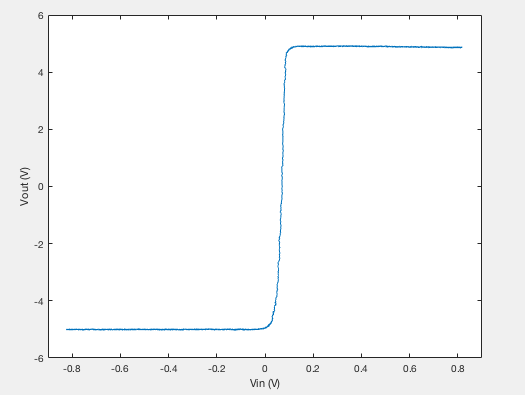
\includegraphics[scale=.40]{ExperimentalImplementation/VTC.png}
				\caption{Experimental range of operation}
				\label{fig:vtc}
			\end{center}
		\end{figure}
		
		The range of operation is extremely narrow. This, however, is expected due to the limits imposed by the use of a cascode current mirror. The cascode affords more gain at the expense of voltage range. This was explored in more depth in Task 3. In order to prevent the op amp from saturating, a 1000:1 voltage divider was added at the signal input. The channel 1 probe was connected after the voltage divider to compensate for the 60dB drop from the voltage divider. Channel 2 was connected at the final output of the operational amplifier.  In order to ensure the op amp was unity gain stable, a 150pF capacitor had to be added to the output node of the common source amplifier stage. Prior to this modification there was no 0 dB gain crossing which meant that op amp was in fact unstable and would oscillate without input. The compensated gain can be seen in Figure \ref{fig:compgain}.
		
		
			\begin{figure}[H]
			\centering
			\begin{subfigure}[b]{0.45\textwidth}
				\centering
		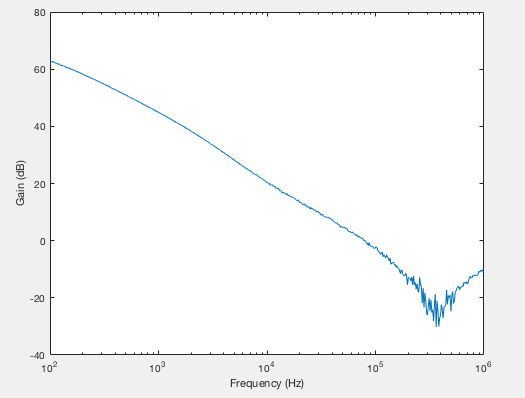
\includegraphics[scale=.40]{ExperimentalImplementation/gainwithcomp.png}
\caption{Gain plot of loaded amplifier and frequency compensation}
\label{fig:gainwithcomp}
			\end{subfigure}
			\hfill
			\begin{subfigure}[b]{0.45\textwidth}
		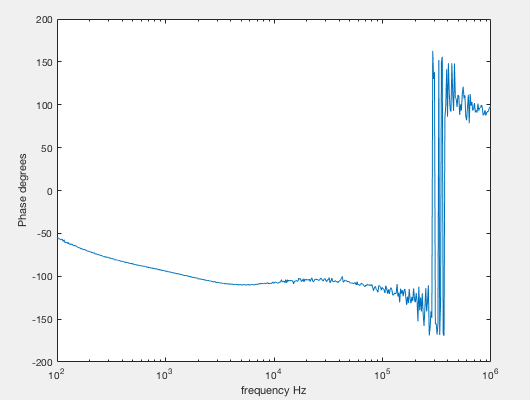
\includegraphics[scale=.40]{ExperimentalImplementation/phasewithcomp.png}
\caption{Phase plot of loaded amplifier with frequency compensation}
\label{fig:phasewithcomp}
			\end{subfigure}
			\caption{Common mode gain, Acm at 1V}
			\label{fig:compgain}
		\end{figure} 
	
	This addition moved the unity gain frequency bandwidth to 170 kHz, which is greater than the required 150kHz.
		
		
		
		
		
		
		
		
		
		
		
		
		
		
		
		
		
		 The final stage output gain with a 500 $\Omega$ load can be seen in Figure \ref{fig:gainwithload}.
				
		
	
	
	\begin{figure}[H]
		\centering
		\begin{subfigure}[b]{0.45\textwidth}
			\centering
			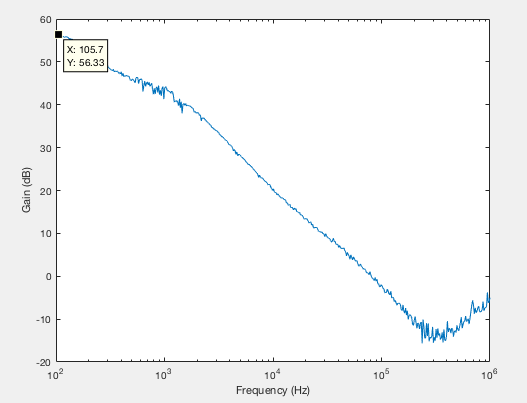
\includegraphics[scale=.40]{ExperimentalImplementation/gainwithload.png}
		\caption{Gain of loaded amplifier}
		\label{fig:tload}
		\end{subfigure}
		\hfill
		\begin{subfigure}[b]{0.45\textwidth}
			\centering
			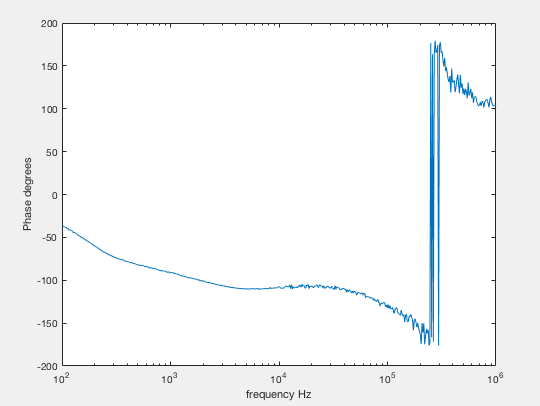
\includegraphics[scale=.40]{ExperimentalImplementation/phasewithload.png}
		\caption{Phase plot of loaded amplifier}
		\label{fig:phasewithload}
		\end{subfigure}
		\caption{Common mode gain, Acm at 1V}
		\label{fig:gainwithload}
	\end{figure} 
	
It can be seen that the gain dropped 3.67dB from the unloaded gain of 60dB. This is slightly out of spec and can be compensated by using an only slighlty larger load of 600 $\Omega$. The op amp did, however, remain stable with the added load.
	
	
	
The op amp was then required to be constructed in two different configurations. One in the inverting configuration and the other in the non-inverting. The experimental schematic for the inverting can be seen in Figure \ref{fig:invertingschem}

		\begin{figure}[H]
	\begin{center}
		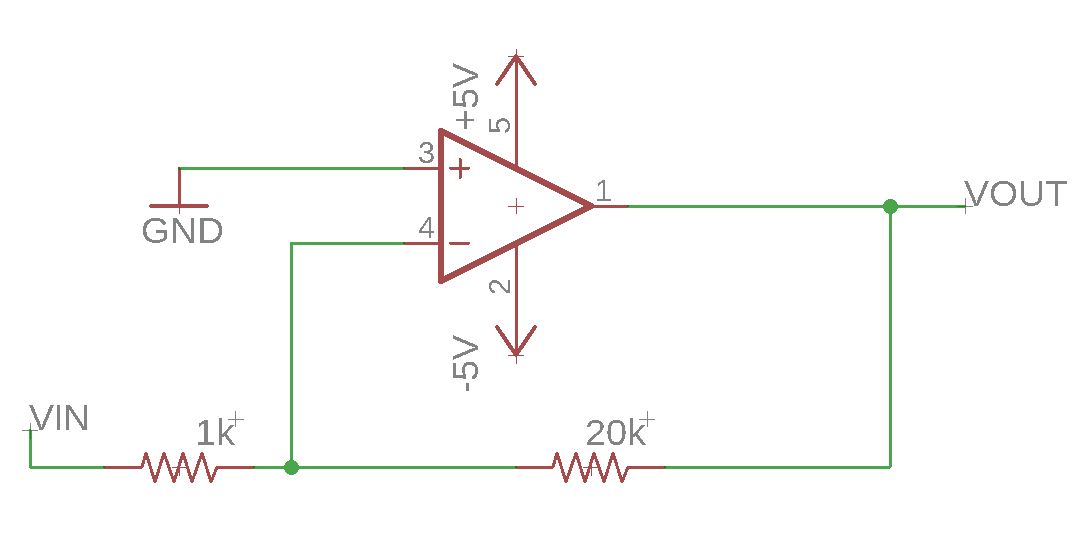
\includegraphics[scale=.40]{ExperimentalImplementation/invertingschem.png}
		\caption{Gain of inverting amplifier}
		\label{fig:invertingschem}
	\end{center}
\end{figure}

The op amp shown is the op amp desgined in prior in Task 4. The ideal gain was is -20 V/V. The measured gain can be seen in Figure \ref{fig:invertinggain}.
	
	
	
				\begin{figure}[H]
		\centering
		\begin{subfigure}[b]{0.45\textwidth}
			\centering
		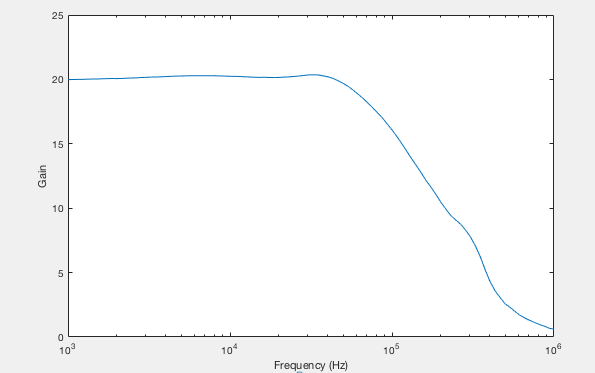
\includegraphics[scale=.40]{ExperimentalImplementation/invertingain.png}
\caption{Gain of inverting amplifier}
\label{fig:invertinggain1}
		\end{subfigure}
		\hfill
		\begin{subfigure}[b]{0.45\textwidth}
			\centering
		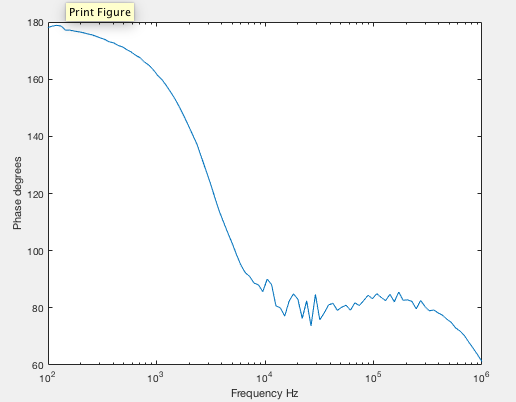
\includegraphics[scale=.40]{ExperimentalImplementation/invertingphase.png}
\caption{Phase plot of inverting amplifier}
\label{fig:invertingphase}
		\end{subfigure}
		\caption{Common mode gain, Acm at 1V}
		\label{fig:invertinggain}
	\end{figure} 




	
The gain can be seen to be 27dB, when converted to V/V is found to be -23 V/V. This is slightly larger than what was expected in the ideal case. It should be noted that the negattive sign of this measurement comes from the fact that the phase plot starts at 180$^\circ$ phase. Notably, this configuration seems to have driven the op amp back into instability with the dissappearance of the 0dB crossing. The spectrum plot for the inverting configuration can be seen in Figure \ref{fig:spectrum}.

		\begin{figure}[H]
	\begin{center}
		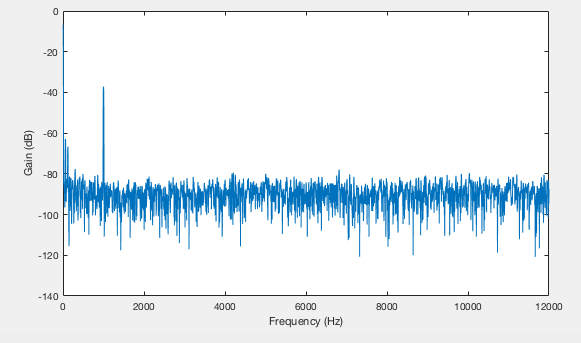
\includegraphics[scale=.40]{ExperimentalImplementation/spectrum.png}
		\caption{Harmonic spectrum of amplifier}
		\label{fig:spectrum}
	\end{center}
\end{figure}

This was generated by inputting a 100mV$_{pp}$ signal at 1kHz. The second harmonic was undiscernable with only the 1kHz having any meaningful amplitude.  Finally op amp was configured for non inverting output. This topology can be seen in Figure \ref{fig:noninvertingschem}
		
						\begin{figure}[H]
			\begin{center}
				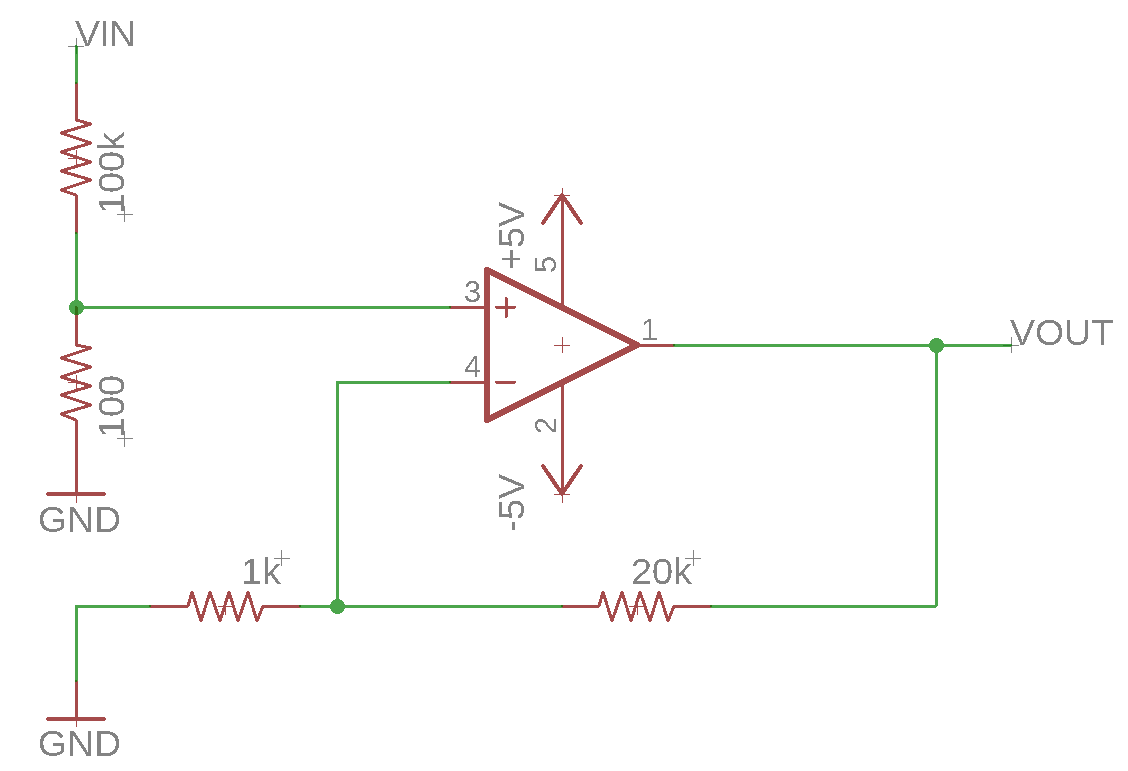
\includegraphics[scale=.40]{ExperimentalImplementation/noninvertingschem.png}
				\caption{Gain of non-inverting amplifier}
				\label{fig:noninvertingschem}
			\end{center}
		\end{figure}
	
This configuration should, under ideal operation, provide 21V/V  of gain. The measured gain can be seen in Figure \ref{fig:gainnoninverting}.
		
		
		
						\begin{figure}[H]
			\centering
			\begin{subfigure}[b]{0.45\textwidth}
				\centering
				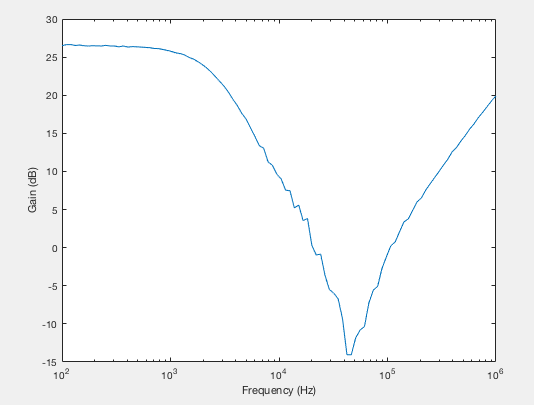
\includegraphics[scale=.40]{ExperimentalImplementation/gainnoninverting.png}
\caption{Gain of non-inverting amplifier}
\label{fig:gainnoninverting1}
			\end{subfigure}
			\hfill
			\begin{subfigure}[b]{0.45\textwidth}
				\centering
			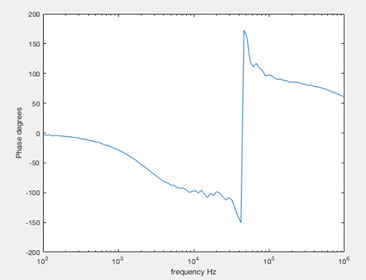
\includegraphics[scale=.40]{ExperimentalImplementation/phasenoninverting.png}
\caption{Phase plot of non-inverting amplifier}
\label{fig:phasenoninverting}
			\end{subfigure}
			\caption{Common mode gain, Acm at 1V}
			\label{fig:gainnoninverting}
		\end{figure} 
		
The measured gain was nearly 27dB and when converted to V/V yields 23.8 V/V.  This larger than the predicted 21 V/V but with the correct phase of 0. Notably, this configuration remained stable.



	\end{document}
	